%! TEX root = ../../main.tex

\chapter{Preliminaries: Factorized Machine Learning}
\label{chapter:preliminary}

This chapter details the preliminary theoretical concepts for this thesis. First, we explain \hyperref[sec:2-data-integration]{Data Integration}: the process of combining data from different sources, which is crucial to any ML workflow. With these concepts in mind, we explore \hyperref[sec:2-factorized-ml]{Factorized Machine Learning} in detail. Finally, in \autoref{sec:2-ml-on-gpu}, we explain GPUs and how they are crucial for the ML industry. With these concepts, we provide the theoretical foundation necessary for understanding the content presented in the next chapters of this thesis.


\section{Data Integration}
\label{sec:2-data-integration}
To grasp the value and intricacies of Factorized ML, one first needs to understand the field of Data Integration (DI). In the broadest definition, DI details relations between data(sets), allowing data from disparate sources to be consolidated into a single dataset. This is essential for ML use cases, as ML libraries (e.g., Keras\footnote{\url{https://keras.io/}}, TensorFlow\footnote{\url{https://www.tensorflow.org/}}) expect a single table as input. An example of such a DI scenario is shown in \autoref{fig:running-example-fac-vs-mat}.

% Paragraph on formalization?

However, while joining datasets to a single table is necessary for ML, it can introduce major overheads \cite{data-management-in-ML-kumar-2017}:

\begin{enumerate}
    \item \textbf{Extra storage}\\ The joined dataset will take extra space to store.
    \item \textbf{Computational redundancy} \\ Joining tables can introduce duplication of values in the materialized data (shown in orange in \autoref{fig:running-example-fac-vs-mat}). These values are included in any computations done during the training of an ML model in this dataset, resulting in duplicate computations.
    \item \textbf{Join time} \\For complex scenarios, joining datasets can take a significant amount of time.
    \item \textbf{Maintenance headaches} \\Join query needs updating when changing input table schemas.
\end{enumerate}

Factorized Machine Learning aims to alleviate problems one to three by “learning over joins” \cite{orion_learning_gen_lin_models}, that is, pushing the computations needed for an ML model down to the separate tables.

\subsection{Schema Mapping}
Schema mapping is an integral step to the Data Integration process, and thus to Factorized ML. These mappings specify how the source datasets map to the target tables. Having a formal way of specifying how these datasets relate is especially important for factorized ML. It allows us to convert these relationships between the source tables and the target table to a form that can be translated to linear algebra: the normalized matrix (detailed in \autoref{subsec:2-normalized-matrix}).

The language used for these mappings is \textit{source-to-target tuple generating dependencies (s-t tgd)} \cite{tgds-Fagin2009}. These are formulas in first-order logic form that specify, through atomic formulas over schemas $S$ and the target schema $T$, how the tuples from the source tables map to the target table. Here, we show the TGD for the running example.\begin{alignat*}{2}
    \intertext{Given source datasets, with abbreviated column names:}
     & o=order\_id, c=customer\_id, d=date,                                                                                                                      \\
     & p_{id}=product\_id, q=quantity, p=price, rq=return\_quantity                                                                                              \\
     & S_1(o, c, d)                                                                                                                                              \\
     & S_2(o, p_{id} , q,  p)                                                                                                                                    \\
     & S_3(o, p_{id}, rq)                                                                                                                                      & \\
    \intertext{the mapping to target table $T$ can be specified as follows. First we left join $S_2$ with $S_3$:}
     & \forall o, p_{id}, q, p, rq \left( S_3(o, p_{id}, rq) \land S_2(o, p_{id}, q, p) \rightarrow \exists o, p_{id}, q, p, rq T(o, p_{id}, q, p, rq) \right)   \\
    \intertext{Next, we inner join the result with $S_1$ to get the final schema $T(o, c, d, p_{id}, q, p, rq)$:} \begin{split}
                                                                                                                      & \forall o, c, d, p_{id}, q, p, rq ( S_1(o, c, d) \land T(o, p_{id}, q, p, rq) \rightarrow \\
                                                                                                                      & \exists o, c, d, p_{id}, q, p, rq T(o, c, d, p_{id}, q, p, rq) )
                                                                                                                  \end{split}
\end{alignat*}

Now that we have the schema mapping we can translate this to the normalized matrix, which we will do in the next section.

\section{Factorized Machine Learning}
\label{sec:2-factorized-ml}
As stated previously in this thesis, Factorized ML is the process of training Machine Learning models on multiple tables without the need to materialize the join between these tables. This section will go in-depth on how this can be achieved, continuing the running example from \autoref{fig:running-example-fac-vs-mat}.  We start with the definitions (\autoref{subsec:2-normalized-matrix}) followed by an in-depth example of the involved linear algebra (\autoref{subsubsec:2-fac-ml-example}).

\subsection{Normalized Matrix}
\label{subsec:2-normalized-matrix}

As Machine Learning Algorithms can be expressed in Linear Algebra (LA) we need to express the Data Integration scenario of an ML use case in terms of Linear Algebra, .i.e., we need to translate the Schema Mappings of an integration scenario to Linear Algebra to allow us to achieve the goal of “pushing down” ML to the separate source tables. This is achieved through the \textbf{ Normalized matrix}: A set of matrices that capture the necessary DI metadata telling us how the source tables map to the materialized Target table \cite{amalur, morpheus}.

The \textbf{Mapping matrix} and \textbf{Indicator matrix} respectively represent how the columns and rows from each source table $S_k$ map to the Target table $T$.

\subsubsection{Mapping Matrix}
The Mapping Matrix $M$ is a set of matrices $M_k$ for each source table $S_k$ that denotes how source columns map to target columns. A value of 1 in this matrix denotes that the corresponding column (via column number) in $S_k$ corresponds to the corresponding column (via column number) in $T$. The formal definition is as follows.

\begin{definition}[\textit{Mapping matrix} \cite{amalur}]
    Each source table $S_k$ has a corresponding binary Mapping matrix $M$ of shape $c_T \times c_{S_k}$, where
    \begin{align*}
        M_k[i,j] = \begin{cases}
                       1, & \text{if $j$-th column of $S_k$ is mapped to the $i$-th column of $T$} \\
                       0, & \text{otherwise}
                   \end{cases}
    \end{align*}
\end{definition}

Note that in the case that there is no column overlap between source tables this Mapping Matrix is redundant. This does affect how materialization works, as shown in \autoref{def:materialization}.


\subsubsection{Indicator Matrix}
% TODO intro
Now that we have defined how to map the columns from source tables to target table, we need to do the same for the rows. This is done with the \textbf{Indicator} matrix.

\begin{definition}[\textit{Indicator matrix} \cite{morpheus}]
    Each source table $S_k$ has a corresponding binary Indicator matrix $I$ of shape $r_T \times r_{S_k}$, where
    \begin{align*}
        I_k[i,j] = \begin{cases}
                       1, & \text{if $i$-th row of $S_k$ is mapped to the $j$-th row of $T$} \\
                       0, & \text{otherwise}
                   \end{cases}
    \end{align*}
\end{definition}

% \subsubsection{Redundancy Matrix}


\subsubsection{Materialization}
Using the normalized matrix, we can now \textbf{materialize} the join to get the Target matrix $T$:

\begin{definition}[\textit{Materializing the Normalized Matrix to obtain Target matrix $T$}]
    \begin{itemize}
        \item[]
        \item[] Given
        \item[$k$] Table id $k \in [1,n]$
        \item[$S_k$] Source tables
        \item[$M_k$] Mapping matrices
        \item[$I_k$] Indicator matrices
    \end{itemize}
    \[
        T = \begin{cases}
            \sum_{k=1}^n  I_k S_k M^T_k,  & \text{if there is column overlap between source tables} \\
            \begin{bNiceMatrix}
                \vdots  & \vdots & \vdots  \\
                I_1 S_1 & \cdots & I_n S_n \\
                \vdots  & \vdots & \vdots  \\
            \end{bNiceMatrix}, & \text{otherwise}
        \end{cases}
    \]
    \label{def:materialization}

\end{definition}

The materialization case when there is no column overlap is a horizontal concatenation of each source matrix $S_k$ multiplied by $I_k$: $I_k S_k, k \in [1,n]$. Intuitively the materialization process can be seen as:
\begin{algorithmic}
    \ForEach {$k \in [1,n]$} \Comment{For each source table}
    \State $rows_k \gets I_k S_k$ \Comment{Map the source table rows to the target table}
    \State $T_k \gets rows_k M^T_k$ \Comment{Map the source table columns to the target table}
    \EndFor
    \State $T \gets \sum_{k=0}^{n-1} T_k$ \Comment{Sum the results}
\end{algorithmic}

\subsubsection{Running Example: Normalized Matrix}
\label{subsubsec:2-fac-ml-example}
To make the translation to how the normalized matrix is used in ML algorithms we first show the full normalized matrix of the running example, followed by the materialized Target table $T$. The goal is to show how the matrices interact to allow computation with all information without necessarily materializing the join. For completeness, we show the calculations with the Mapping matrices $M_k$ included, but as highlighted before this is not needed due to this scenario having no column overlap. However, it is insightful to show as it gives an idea of how this process looks when there is column overlap.
\begin{alignat*}{6}
    \intertext{
        These are the corresponding Source matrices $S_{1..3}$ for the source tables shown in \autoref{fig:running-example-fac-vs-mat}. The \textcolor{BurntOrange}{orange} numbers over the columns denote in which column of $T$ they will end up. The \textcolor{RoyalBlue}{blue} numbers at the end of each row illustrate to which target table rows they are mapped.
    }
                                                            & S_1 &     & =
    \begin{bNiceMatrix}[first-row,last-col]
        0 & 1  & 2    &     \\
        1 & 11 & 2024 & 0,1 \\
        2 & 12 & 2024 & 2   \\
        3 & 11 & 2024 & 3   \\
    \end{bNiceMatrix}   \quad                 &     & S_2 &   & =
    \begin{bNiceMatrix}[first-row,last-col]
        3 & 4  & 5  &   \\
        2 & 20 & 40 & 0 \\
        1 & 25 & 25 & 1 \\
        3 & 13 & 39 & 2 \\
        1 & 10 & 10 & 3 \\
    \end{bNiceMatrix}           \quad                 &     & S_3 &   & =
    \begin{bNiceMatrix}[first-row,last-col]
        6 &   \\
        1 & 3 \\
    \end{bNiceMatrix}                                  \\
    \intertext{
        The Indicator matrices denote how rows from $S$ map to rows in $T$. The column number denotes the row in $S$, the row number denotes the row in $T$. The \textcolor{RoyalBlue}{blue} annotations show more clearly how this works in the form \textcolor{RoyalBlue}{row number in $S_k \rightarrow$ row number in $T$}.
    }
                                                            & I_1 &     & =
    \begin{bNiceMatrix}[last-col]
        1 & 0 & 0 & 0 \rightarrow 0 \\
        1 & 0 & 0 & 0 \rightarrow 1 \\
        0 & 1 & 0 & 1 \rightarrow 2 \\
        0 & 0 & 1 & 2 \rightarrow 3 \\
    \end{bNiceMatrix}   \quad                          &     & I_2 &   & =
    \begin{bNiceMatrix}[last-col]
        1 & 0 & 0 & 0 & 0 \rightarrow 0 \\
        0 & 1 & 0 & 0 & 1 \rightarrow 1 \\
        0 & 0 & 1 & 0 & 2 \rightarrow 2 \\
        0 & 0 & 0 & 1 & 3 \rightarrow 3 \\
    \end{bNiceMatrix}     \quad                      &     & I_3 &   & =
    \begin{bNiceMatrix}[last-col]
        0 & \rightarrow 0   \\
        0 & \rightarrow 1   \\
        0 & \rightarrow 2   \\
        1 & 0 \rightarrow 3 \\
    \end{bNiceMatrix}                                            \\
    \intertext{
        The Mapping matrices denote how columns from $S$ map to columns in $T$. The row number denotes the column in $T$, the column number denotes the column in $S$. The \textcolor{BurntOrange}{orange} annotations show this in the form: \textcolor{BurntOrange}{column number in $S_k \rightarrow$ column number in $T$}.
    }
                                                            & M_1 &     & =
    \begin{bNiceMatrix}[last-col]
        1 & 0 & 0 & \textcolor{BurntOrange}{0 \rightarrow 0} \\
        0 & 1 & 0 & \textcolor{BurntOrange}{1 \rightarrow 1} \\
        0 & 0 & 1 & \textcolor{BurntOrange}{2 \rightarrow 2} \\
        0 & 0 & 0 & \textcolor{BurntOrange}{\rightarrow 3}   \\
        0 & 0 & 0 & \textcolor{BurntOrange}{\rightarrow 4}   \\
        0 & 0 & 0 & \textcolor{BurntOrange}{\rightarrow 5}   \\
        0 & 0 & 0 & \textcolor{BurntOrange}{\rightarrow 6}   \\
    \end{bNiceMatrix}   \quad &     & M_2 &   & =
    \begin{bNiceMatrix}[last-col]
        0 & 0 & 0 & \textcolor{BurntOrange}{\rightarrow 0}   \\
        0 & 0 & 0 & \textcolor{BurntOrange}{\rightarrow 1}   \\
        0 & 0 & 0 & \textcolor{BurntOrange}{\rightarrow 2}   \\
        1 & 0 & 0 & \textcolor{BurntOrange}{0 \rightarrow 3} \\
        0 & 1 & 0 & \textcolor{BurntOrange}{1 \rightarrow 4} \\
        0 & 0 & 1 & \textcolor{BurntOrange}{2 \rightarrow 5} \\
        0 & 0 & 0 & \textcolor{BurntOrange}{\rightarrow 6}   \\
    \end{bNiceMatrix} \quad &     & M_3 &   & =
    \begin{bNiceMatrix}[last-col]
        0 & \textcolor{BurntOrange}{\rightarrow 0}   \\
        0 & \textcolor{BurntOrange}{\rightarrow 1}   \\
        0 & \textcolor{BurntOrange}{\rightarrow 2}   \\
        0 & \textcolor{BurntOrange}{\rightarrow 3}   \\
        0 & \textcolor{BurntOrange}{\rightarrow 4}   \\
        0 & \textcolor{BurntOrange}{\rightarrow 5}   \\
        1 & \textcolor{BurntOrange}{0 \rightarrow 6} \\
    \end{bNiceMatrix}
\end{alignat*}
\begin{gather*}
    \begin{alignat*}{4}
        \intertext{For conciseness we show the calculation of one of the sub-target tables $T_1$.}
                            & T_1 &       & = I_1                 &  & S_1 &  & M_1^T                   \\
                            & T_1 &       & = \begin{bNiceMatrix}
                                                  1 & 0 & 0 \\
                                                  1 & 0 & 0 \\
                                                  0 & 1 & 0 \\
                                                  0 & 0 & 1 \\
                                              \end{bNiceMatrix} &  &
        \begin{bNiceMatrix}
            1 & 11 & 2024 \\
            2 & 12 & 2024 \\
            3 & 11 & 2024 \\
        \end{bNiceMatrix} &     & M_1^T                                                                 \\
                            & T_1 &       & = \begin{bNiceMatrix}
                                                  1 & 11 & 2024 \\
                                                  1 & 11 & 2024 \\
                                                  2 & 12 & 2024 \\
                                                  3 & 11 & 2023 \\
                                              \end{bNiceMatrix} &  &     &  & \begin{bNiceMatrix}
                                                                                  1 & 0 & 0 & 0 & 0 & 0 & 0 \\
                                                                                  0 & 1 & 0 & 0 & 0 & 0 & 0 \\
                                                                                  0 & 0 & 1 & 0 & 0 & 0 & 0 \\
                                                                              \end{bNiceMatrix} \\
    \end{alignat*}\\
    \hspace{-4cm}
    T_1  = \begin{bNiceMatrix}
        \Block[fill=red!15,rounded-corners]{4-3}{}
        1 & 11 & 2024 & 0 & 0 & 0 & 0 \\
        1 & 11 & 2024 & 0 & 0 & 0 & 0 \\
        2 & 12 & 2024 & 0 & 0 & 0 & 0 \\
        3 & 11 & 2023 & 0 & 0 & 0 & 0 \\
    \end{bNiceMatrix}
\end{gather*}

\begingroup
\setlength{\arraycolsep}{4.5pt}
\begin{alignat*}{2}
    \intertext{
        The materialized Target table $T$ is the element wise sum of the dot product of each tuple of Indicator, Source, and Mapping matrices. For each source table $S_k$ the intermittent result is shown as $T_k$. For clarity the cells from each source table are coloured in the same colour in the intermittent result and in Target table $T$.
    }
     & T_1= I_1 S_1 M_1^T &  & = \begin{bNiceMatrix}[first-row]
                                     0 & 1  & 2    & 3 & \cdots & 6 \\
                                     \Block[fill=red!15,rounded-corners]{4-3}{}
                                     1 & 11 & 2024 & 0 & \cdots & 0 \\
                                     1 & 11 & 2024 & 0 & \cdots & 0 \\
                                     2 & 12 & 2024 & 0 & \cdots & 0 \\
                                     3 & 11 & 2023 & 0 & \cdots & 0 \\
                                 \end{bNiceMatrix}
    T_2= I_2 S_2 M_2^T= \begin{bNiceMatrix}[first-row]
                            0 & 1 & 2 & 3                                             & 4  & 5  & 6 \\
                            0 & 0 & 0 & \Block[fill=blue!15,rounded-corners]{4-3}{} 2 & 20 & 40 & 0 \\
                            0 & 0 & 0 & 1                                             & 25 & 25 & 0 \\
                            0 & 0 & 0 & 3                                             & 13 & 39 & 0 \\
                            0 & 0 & 0 & 1                                             & 10 & 10 & 0 \\
                        \end{bNiceMatrix}
    \\
     & T_3= I_3 S_3 M_3^T &  & = \begin{bNiceMatrix}[first-row]
                                     0 & \cdots & 5 & 6                                              \\
                                     0 & \cdots & 0 & 0                                              \\
                                     0 & \cdots & 0 & 0                                              \\
                                     0 & \cdots & 0 & 0                                              \\
                                     0 & \cdots & 0 & \Block[fill=orange!15,rounded-corners]{1-1}{}1 \\
                                 \end{bNiceMatrix}
    T  = \sum_{k=0}^{2} I_k S_k M^T_k =  \begin{bNiceMatrix}[first-row,last-col]
                                             0 & 1  & 2    & 3                                           & 4  & 5  & 6                                                  \\
                                             \Block[fill=red!15,rounded-corners]{4-3}{}
                                             1 & 11 & 2024 & \Block[fill=blue!15,rounded-corners]{4-3}{}
                                             2 & 20 & 40   & 0                                           & 0                                                            \\
                                             1 & 11 & 2024 & 1                                           & 25 & 25 & 0                                              & 1 \\
                                             2 & 12 & 2024 & 3                                           & 13 & 39 & 0                                              & 2 \\
                                             3 & 11 & 2024 & 1                                           & 10 & 10 & \Block[fill=orange!15,rounded-corners]{1-1}{}1 & 3 \\
                                         \end{bNiceMatrix}
\end{alignat*}
\endgroup


\subsection{Factorized Linear Algebra}
In the previous section we have shown the properties of the Normalized matrix. This section will show how commonly used Linear Algebra operators are rewritten for the Normalized matrix for the purpose of performing factorized ML \cite{morpheus}. We will show how to perform element-wise operations, reduction operations, dot-product operations, and a running example of right matrix multiplication (RMM) on the Normalized matrix. The goal is to show how (most of) these operations can be performed without materializing the join between the source tables, and how the Normalized matrix allows us to do so.


\subsubsection{Element-wise Scalar Operations}
This group of operators all perform an operation on every element of a matrix, independently of one another. The arithmetic operations are: $+$, $-$, $\times$, $\div$ and $ ^\wedge $ (these operators are denoted by $\oslash$). This can be seen as a scalar function $f$ applied to each element of a matrix $T$. The rewrite rule therefore is very simple for these arithmetic operators, as well as for any other scalar function (e.g., $log$, $round$) $f$:
\begin{alignat*}{2}
    x \oslash T & \rightarrow [x \oslash S, I, M] \\
    T \oslash x & \rightarrow [S \oslash x, I, M]
    \intertext{or more generally:}
    f(T)        & \rightarrow [f(S), I, M]
\end{alignat*}

These operations all return a normalized matrix, and can thus be performed without materializing the join between the source tables. In the used implementation \cite{schijndel_cost_estimation}, when a normalized matrix is transposed, the actual computation is not carried out, but the transpose is simply added as a flag. Then for any downstream operators the transpose flag is checked, and the computation is performed accordingly. For these element-wise operations the transposed rewrite is:
\begin{alignat*}{2}
    f(T^T) & \rightarrow [f(S), I, M]^T
\end{alignat*}

\subsubsection{Aggregation}
The supported aggregation operators are row-wise and column-wise summation, respectively abbreviated to rowSums and colSums. For the factorized rowSums case we sum each source table separately, then multiply with the indicator matrices and sum the results, the mapping matrix is irrelevant this operation produces a single (column) vector of size $r_T \times 1$. For the transposed case it is equal to a column summation. These rewrite rules are:
\begin{alignat*}{2}
    \text{rowSums}(T)   & \rightarrow \sum_1^k I_k \text{rowSums}(S_k) \\
    \text{rowSums}(T^T) & \rightarrow \text{colSums}(T)
\end{alignat*}

Summing column wise gives a row vector of shape $1 \times c_T$. It is equal to first summing the indicator tables column=wise, then materializing with these aggregated indicator matrices.  The rewrite rule for the factorized case is:
\begin{alignat*}{2}
    \text{colSums}(T)   & \rightarrow \sum_1^k \text{colSums}(I_k) S_k M_k^T \\
    \text{colSums}(T^T) & \rightarrow \text{rowSums}(T)
\end{alignat*}
As these operations do not create normalized matrices, and in fact materialize (part of) the join the benefit of factorized computation is smaller.

\subsubsection{Multiplication}
As matrix multiplication is not commutative there are different rewrite rules for left- and right-matrix multiplication. The rewrite rule for left matrix multiplication (LMM) with another matrix $X$ is:
\begin{alignat*}{2}
    TX   & \rightarrow \sum_1^k I_k S_k M_k^T X \\
    T^TX & \rightarrow (X^TT)^T
\end{alignat*}

For right matrix multiplication (RMM) the rule is the same, we still essentially materialize the join, but with $X$ on the left-hand side:
\begin{alignat*}{2}
    XT   & \rightarrow \sum_1^k X I_k S_k M_k^T \\
    XT^T & \rightarrow (TX^T)^T
\end{alignat*}


% \todo{Overview table like in Morpheus?}

\subsubsection{Running Example: Right Matrix Multiplication}

\begingroup
\setlength{\arraycolsep}{3.0pt}
\begin{alignat*}{1}
    \intertext{We showcase right RMM and its rewrite rule by multiplying with $X$. First for the materialized Target table $T$:}
    X T & = \begin{bNiceMatrix}
                1 & 1 & 2 & 3 \\
            \end{bNiceMatrix}
    \begin{bNiceMatrix}
        1 & 11 & 2024 & 2 & 20 & 40 & 0 \\
        1 & 11 & 2024 & 1 & 25 & 25 & 0 \\
        2 & 12 & 2024 & 3 & 13 & 39 & 0 \\
        3 & 11 & 2023 & 1 & 10 & 10 & 1 \\
    \end{bNiceMatrix}                                                         \\
        & =\begin{bNiceMatrix}
               15 & 79 & 14165 & 12 & 101 & 173 & 3 \\
           \end{bNiceMatrix}                                             \\
    \intertext{Now for the Normalized matrix, recall the rewrite rule for RMM:}
    X T & = \sum_{k=0}^{n-1} X I_k S_k M^T_k
    \intertext{For conciseness we refer back to sub results $T_{0\cdots2}$ and use them directly here. We also leave out $X$ in the sub calculations for $T_{1,2}$.}
        & = X T_0 + X T_1 + X T_2                                                           \\
        & = \begin{bNiceMatrix}
                1 & 1 & 2 & 3 \\
            \end{bNiceMatrix} \begin{bNiceMatrix}
                                  1 & 11 & 2024 & 0 & \cdots & 0 \\
                                  1 & 11 & 2024 & 0 & \cdots & 0 \\
                                  2 & 12 & 2024 & 0 & \cdots & 0 \\
                                  3 & 11 & 2023 & 0 & \cdots & 0 \\
                              \end{bNiceMatrix} + X \begin{bNiceMatrix}
                                                        0 & 0 & 0 & 2 & 20 & 40 & 0 \\
                                                        0 & 0 & 0 & 1 & 25 & 25 & 0 \\
                                                        0 & 0 & 0 & 3 & 13 & 39 & 0 \\
                                                        0 & 0 & 0 & 1 & 10 & 10 & 0 \\
                                                    \end{bNiceMatrix} + X\begin{bNiceMatrix}
                                                                             0 & \cdots & 0 & 0 \\
                                                                             0 & \cdots & 0 & 0 \\
                                                                             0 & \cdots & 0 & 0 \\
                                                                             0 & \cdots & 0 & 1 \\
                                                                         \end{bNiceMatrix} \\
        & =\begin{bNiceMatrix}
               15 & 79 & 14165 & 0 & 0 & 0 & 0 \\
           \end{bNiceMatrix} +
    \begin{bNiceMatrix}
        0 & 0 & 0 & 12 & 101 & 173 & 0 \\
    \end{bNiceMatrix}+
    \begin{bNiceMatrix}
        0 & 0 & 0 & 0 & 0 & 0 & 3 \\
    \end{bNiceMatrix}                                                               \\& =\begin{bNiceMatrix}
        15 & 79 & 14165 & 12 & 101 & 173 & 3 \\
    \end{bNiceMatrix}
\end{alignat*}
\endgroup

\subsection{Machine Learning Models}
We use the same ML models as \cite{morpheus} and \cite{schijndel_cost_estimation}. The models are: Linear Regression, Logistic Regression, K-means clustering, and Gaussian NMF. As we have shown the rewrite rules for the used Linear Algebra operators, we can now show how these models can be rewritten for the Normalized matrix. This allows us to perform these ML models without materializing the join between the source tables. The algorithms are shown in the following sections, and the used factorized operators are \red{highlighted in red}. In the algorithms we use the following notation: $X$ is the matrix of independent variables, in our case the normalized matrix. $y$ is the dependent variable, and $w$ is the weight vector. $\gamma$ is the learning rate, and $n$ is the number of iterations.

\subsubsection{Linear Regression}
\begin{algorithm}[ht!]
    \caption[Linear regression]{Linear regression using Gradient Descent
        \cite{morpheus}}\label{alg:linear-regression}
    \begin{algorithmic}
        \Require $X, y , w, \gamma$
        \For{$i \in 1:n$}
        \State $w = w - \gamma (\text{\red{$X^T$}}((\text{\red{$X w$}}) - y))$
        \EndFor
    \end{algorithmic}
\end{algorithm}
Linear Regression (\autoref{alg:linear-regression}) is an ML technique fit for finding linear relationships between independent variables and a dependent variable. The used implementation utilizes gradient descent to gradually approach the optimal solution. As seen in the algorithm, the used LA operators on the normalized matrix $T$ are Transpose $T^T$, and Left Matrix Multiplication $TX$.

\subsubsection{Logistic Regression}
Logistic Regression (\autoref{alg:logistic-regression}) is very similar to Linear Regression, but instead of predicting a continuous value, it predicts a binary value. The rewrite rule for Logistic Regression uses the same operators as Linear Regression: Transpose and Left Matrix Multiplication.

\begin{algorithm}[ht]
    \caption[Linear regression]{Logistic regression using Gradient Descent
        \cite{morpheus}}\label{alg:logistic-regression}
    \begin{algorithmic}
        \Require $X, y , w, \gamma$
        \For{$i \in 1:n$}
        \State $w = w - \gamma \left(\text{\red{$X^T$}} \frac{y}{1+e^{\text{\red{$X w$}}}}\right)$
        \EndFor
    \end{algorithmic}
\end{algorithm}

\subsubsection{K-means Clustering}
The previously mentioned regression algorithms are supervised, i.e., they predict a value based on a set of input features. K-means clustering is an unsupervised algorithm, which groups data points into, a predefined number of, clusters based on their similarity. The operators used to compute the clusters are $exp$ ($X^2$), Scalar Multiplication, Transposition, Row Summation and Left Matrix Multiplication. The algorithm is shown in \autoref{alg:k-means}.

\begin{algorithm}[ht]
    \caption[K-Means Clustering]{K-Means Clustering
        \cite{morpheus}\\
        $\mathbf{1}_{r \times c}$ denotes a matrix of size $r \times c$ filled with ones, this is used to repeat a vector to a matrix, either row- or column-wise.}\label{alg:k-means}
    \begin{algorithmic}
        \Require $X, k$ (number of centroids)
        \State $C = \text{rand}(r_X \times k)$ \Comment{Randomly initialize centroids matrix $C$}
        \State $D_X = \text{\red{rowSums($X^2$)}} \times \mathbf{1}_{1 \times k}$ \Comment{Compute the $l^2$-norm of points for distances}
        \State $T_2 = \text{\red{$2 \times X$}}$

        \For{$i \in 1:n$}
        \State $D = D_X - T_2C + \left( \mathbf{1}_{r_X\times 1} \times \text{colSums}(C^2) \right)$ \Comment{Compute distances}
        \State $A = (D == \text{rowMin}(D) \times \mathbf{1}_{1 \times k})$ \Comment{Assign points to the closest centroid}
        \State $C =\frac{\text{\red{$X^T A$}}}{\mathbf{1}_{c_X \times 1} \times \text{colSums}(A)}$ \Comment{Update centroids}
        \EndFor
    \end{algorithmic}
\end{algorithm}

\subsubsection{Gaussian Non-negative Matrix Factorization}
Gaussian Non-negative Matrix Factorization (Gaussian NMF) is a technique used to decompose a matrix into two, smaller, non-negative matrices. It is used for feature extraction from data, and is often used in image processing and text mining. The operators used in the algorithm are Transpose and Right Matrix Multiplication. The rank hyperparameter $r$ controls the size of the resulting matrices. The algorithm is shown in \autoref{alg:gaussian-nmf}.

\begin{algorithm}[ht]
    \caption[Gaussian NMF]{Gaussian Non-negative Matrix Factorization
        \cite{morpheus}}\label{alg:gaussian-nmf}
    \begin{algorithmic}
        \Require $X, r\ \text{(rank)}$
        \State $W = \text{rand}(r_X \times r)$ \Comment{Randomly initialize $W$}
        \State $H = \text{rand}(r \times c_X)$ \Comment{Randomly initialize $H$}
        \For{$i \in 1:n$}
        \State $H = H \times \left(\frac{\text{\red{$W^T X$}}}{W^T W H}\right)$
        \State $W = W \times \left(\frac{\text{\red{$X H^T$}}}{W(H H^T)}\right)$
        \EndFor
    \end{algorithmic}
\end{algorithm}


\subsection{Overview}
\label{subsec:factorized-ml-summary}
In this section we have shown the rewrite rules for the Normalized matrix for commonly used Linear Algebra operators, and how these are used to train Machine Learning models without materializing the join between the source tables. \autoref{tab:factorized-ml-operators-overview} shows an overview of the discussed operators, the last column summarizes the used operators for each ML model. This already shows a reason why a good cost model is necessary for factorized ML, as the different models use a diverse set of operators they benefit in, different ways from factorized computation.

\begin{table}[ht]
    \small
    \resizebox{\textwidth}{!}{%
        % LTeX: enabled=false
\begin{tabular}{p{0.12\linewidth}p{0.16\linewidth}p{0.1\linewidth}p{0.13\linewidth}p{0.15\linewidth}p{0.19\linewidth}}
\toprule
Group & Operator & Example & 2\textsuperscript{nd} Operand & Output & Used in models \\
\midrule\midrule
\multirow[t]{5}{*}{\parbox{1\linewidth}{\vspace{2.3cm}\hspace{0pt}Element-wise}} & Addition & $T + x$ & scalar $x$ & \multirow[t]{5}{*}{\parbox{1\linewidth}{\vspace{2.3cm}Normalized Matrix}} & — \\

 & Multiplication & $T \times x$ & scalar $x$ &  & K-Means \\

 & Division & $T / x$ & scalar $x$ &  & — \\

 & Transposition & $T^T$ & — &  & LinReg, LogReg, K-Means, G-NMF \\

 & Generic Scalar Function & $f(T)$ & f &  & K-Means ($exp$) \\
\cline{1-6}
\multirow[t]{2}{*}{\parbox{1\linewidth}{\vspace{1.3cm}\hspace{0pt}Aggregation}} & Row Summation & \hspace{0pt} row-Sums$(T)$ & — & Column Vector & K-Means \\

 & Column Summation & \hspace{0pt} col-Sums$(T)$ & — & Row Vector & — \\
\cline{1-6}
\multirow[t]{2}{*}{\parbox{1\linewidth}{\vspace{1.3cm}\hspace{0pt}Multiplication}} & Left Matrix Multiplication & $T Y$ & Matrix Y $(c_T \times r_Y)$ & Matrix $(r_T \times c_X)$ & LinReg, LogReg, K-Means \\

 & Right Matrix Multiplication & $Y T$ & Matrix Y $(c_X \times r_X)$ & Matrix $(r_Y \times c_T)$ & G-NMF \\
\cline{1-6}
\bottomrule
\end{tabular}
}
    \caption{Overview of factorized ML operators.}
    \label{tab:factorized-ml-operators-overview}
\end{table}

\section{Machine Learning on GPUs}
\label{sec:2-ml-on-gpu}
Graphics Processing Units (GPUs) have become the processing unit of choice in the field of Machine Learning, as they offer substantial advantages over Central Processing Units (CPUs) for ML. As CPUs are designed for general-purpose needs, this is to be expected. Whereas CPUs excel in sequential tasks like running an operating system, GPUs are designed for parallel tasks. This choice makes them excellent at performing the same operation on many pieces of data at once, exactly what is needed for the prevalent linear algebra operations in ML.

Because GPUs have the upper hand in ML tasks this, thesis focuses on the trade-off between materialization and factorization on GPUs. In this section we will lay out the necessary background information on why GPUs are so well-suited for ML tasks (\autoref{subsec:gpu-architecture}), and how performance of a given task on a GPU can be estimated in (\autoref{subsec:gpu-performance}).

\subsection{Architecture}
\label{subsec:gpu-architecture}

\begin{figure}[ht]
    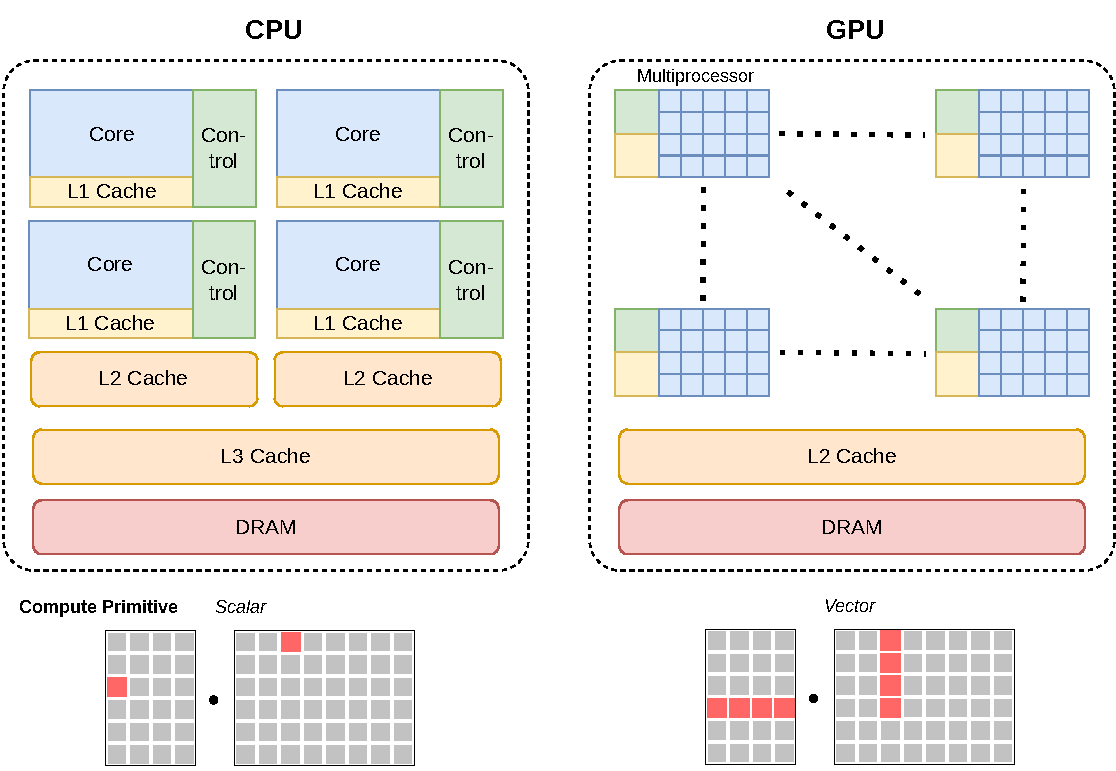
\includegraphics[width=.95\linewidth]{chapters/02_preliminaries/figures/CPU-vs-GPU.pdf}
    \caption[Simplified view of the difference in architecture between a CPU and a GPU.]{ Simplified view of the difference in architecture between a CPU and a GPU. Compute cores are blue, control units green and L1 Cache is marked in yellow. Figure based on visualizations from \cite{gpu-in-ml-survey, cuda-programming-guide, tvm}.}
    \label{fig:cpu-vs-gpu}
\end{figure}
This section details the architecture of a GPU, focussing on what makes it so efficient for Linear Algebra operations. \autoref{fig:cpu-vs-gpu} shows a schematic representation of the difference in architecture between a CPU and a GPU and will be used as a reference for this section.

The heart of the GPU is the Streaming Multiprocessor (SM), which is responsible for executing thousands of parallel threads. Each SM contains several CUDA cores (marked in blue), similar to the cores in a CPU, which perform arithmetic operations. These cores are designed to handle multiple operations simultaneously, making them highly efficient for the matrix and vector computations that are fundamental to Machine Learning.

Data and code move to the SMs through multiple layers of memory. Data is loaded from the host into the GPU's DRAM, from where it moves to the SM through the L2 cache. This facilitates quick data exchange and reduces latency. Threads are organized into blocks, which are then scheduled on SMs. This organization allows for efficient management of resources and execution of threads in parallel. Each SM gets assigned a block of threads, which it then schedules for execution. The cores then execute these threads concurrently resulting in a high degree of parallelism. This processing of multiple data points at a time is called Single Instruction, Multiple Data (SIMD) architecture, which is particularly advantageous for Machine Learning tasks, where the same operation is often applied across many data points. This difference in parallelism is visualized in the bottom part of \autoref{fig:cpu-vs-gpu}. Where a CPU can compute a scalar operation in a single clock cycle, a GPU can perform operations on vectors in parallel.

\subsection{Estimating GPU Performance}
\label{subsec:gpu-performance}
Following the architecture overview, it is essential to understand the performance dynamics of a GPU when applied to Machine Learning tasks, especially the involved Linear Algebra. The GPU's ability to execute thousands of threads concurrently is the basis of its computational power, particularly for tasks with high arithmetic intensity. The following paragraphs draw insights from \cite{nvidia-gpu-performance:online}.

Arithmetic intensity is a measure of the number of math operations performed per memory operation. In the context of GPUs, it is a critical factor in determining performance limitations. A function's execution time on a GPU can be limited by memory bandwidth, math bandwidth, or latency. To conceptualize this, imagine a function that reads data, performs computations, and writes results. The time spent on memory operations $ T_{mem} $ and math operations $ T_{math} $ can overlap, with the total execution time being the maximum of the two: $ \max(T_{mem}, T_{math})$. Due to CPU's inherent sequential nature the total execution time will be much closer to the sum of $T_{mem} \text{ and } T_{math}$. This makes estimating runtime on CPUs easier than for GPUs, as there are some caveats to estimating $T_{mem}$ and $T_{math}$ on GPUs which we will discuss next.

When $ T_{math} $ exceeds $ T_{mem} $, a function is considered math-bound, indicating that the GPU's computational resources are the bottleneck. On the contrary, if $ T_{mem} $ is greater, it is memory-bound, meaning the memory bandwidth is the constraining factor. This relationship is expressed through the inequality $ \frac{\# ops}{BW{math}} > \frac{\# bytes}{BW{mem}} $, which can be rearranged to $ \frac{\# ops}{\# bytes} > \frac{BW{math}}{BW{mem}} $. Here, the left-hand side represents a function's arithmetic intensity, and the right side is the GPU's $ops:byte$ ratio, i.e., the number of Floating Point Operations (FLOPs) per byte accessed from memory.

In practice, many Machine Learning operations, such as linear layers or activation functions, have low arithmetic intensities, often performing just a single operation for every two-byte element read from and written to memory2. This characteristic typically makes them memory-bound on GPUs. However, for operations with high arithmetic intensity, like large matrix multiplications, the GPU's math bandwidth becomes the limiting factor.

To fully leverage a GPU's capabilities, it is crucial to ensure sufficient parallelism. This is achieved by launching a significant number of thread blocks, ideally several times higher than the number of SMs, to minimize the tail effect where only a few active thread blocks remain towards the end of a function's execution. By maintaining a high level of parallelism, GPUs can effectively hide instruction latency and maximize throughput, making them more well-suited for the parallel computations required in Machine Learning than CPUs.
